\chapter{Deep Reinforcement Learning Model}
\label{c:drl}
\section{Overview}
Deep Reinforcement Learning (DRL) combines reinforcement learning (RL) and deep learning. DRL archive remarkable results in many fields, including gaming\cite{mnih2013playing} and robotics\cite{levine2016end}. 
\par 
There are many well-known DRL algorithms including: 
\begin{itemize}
    \item Deep Q-Nnetworks (DQN) \cite{mnih2013playing}
    \item Trust Region Policy Optimization (TRPO) \cite{schulman2015trust}
    \item Proximal Policy Optimization (PPO) \cite{schulman2017proximal}
    \item Deep Deterministic Policy Gradient (DDPG) \cite{silver2014deterministic}
    \item Twin Delayed DDPG (TD3) \cite{fujimoto2018addressing}
    \item Soft Actor-Critic (SAC) \cite{haarnoja2018soft} 
\end{itemize}

We will go through some main characteristics of DRL algorithm and identify the one suites us best from the list above.

\section{Reinforcement Learning (RL)}
RL is a machine learning technique that simulates an agent interacting with the environment. Typical scenario:
    \begin{enumerate}
        \item The agent observes the states from the environment.
        \item The agent performs the action on the environment based on the state observed.
        \item The environment feedback rewards to the agent based on the action performed; the agent will adjust its behavior based on the reward. 
    \end{enumerate}
\begin{figure}[ht]
  \centering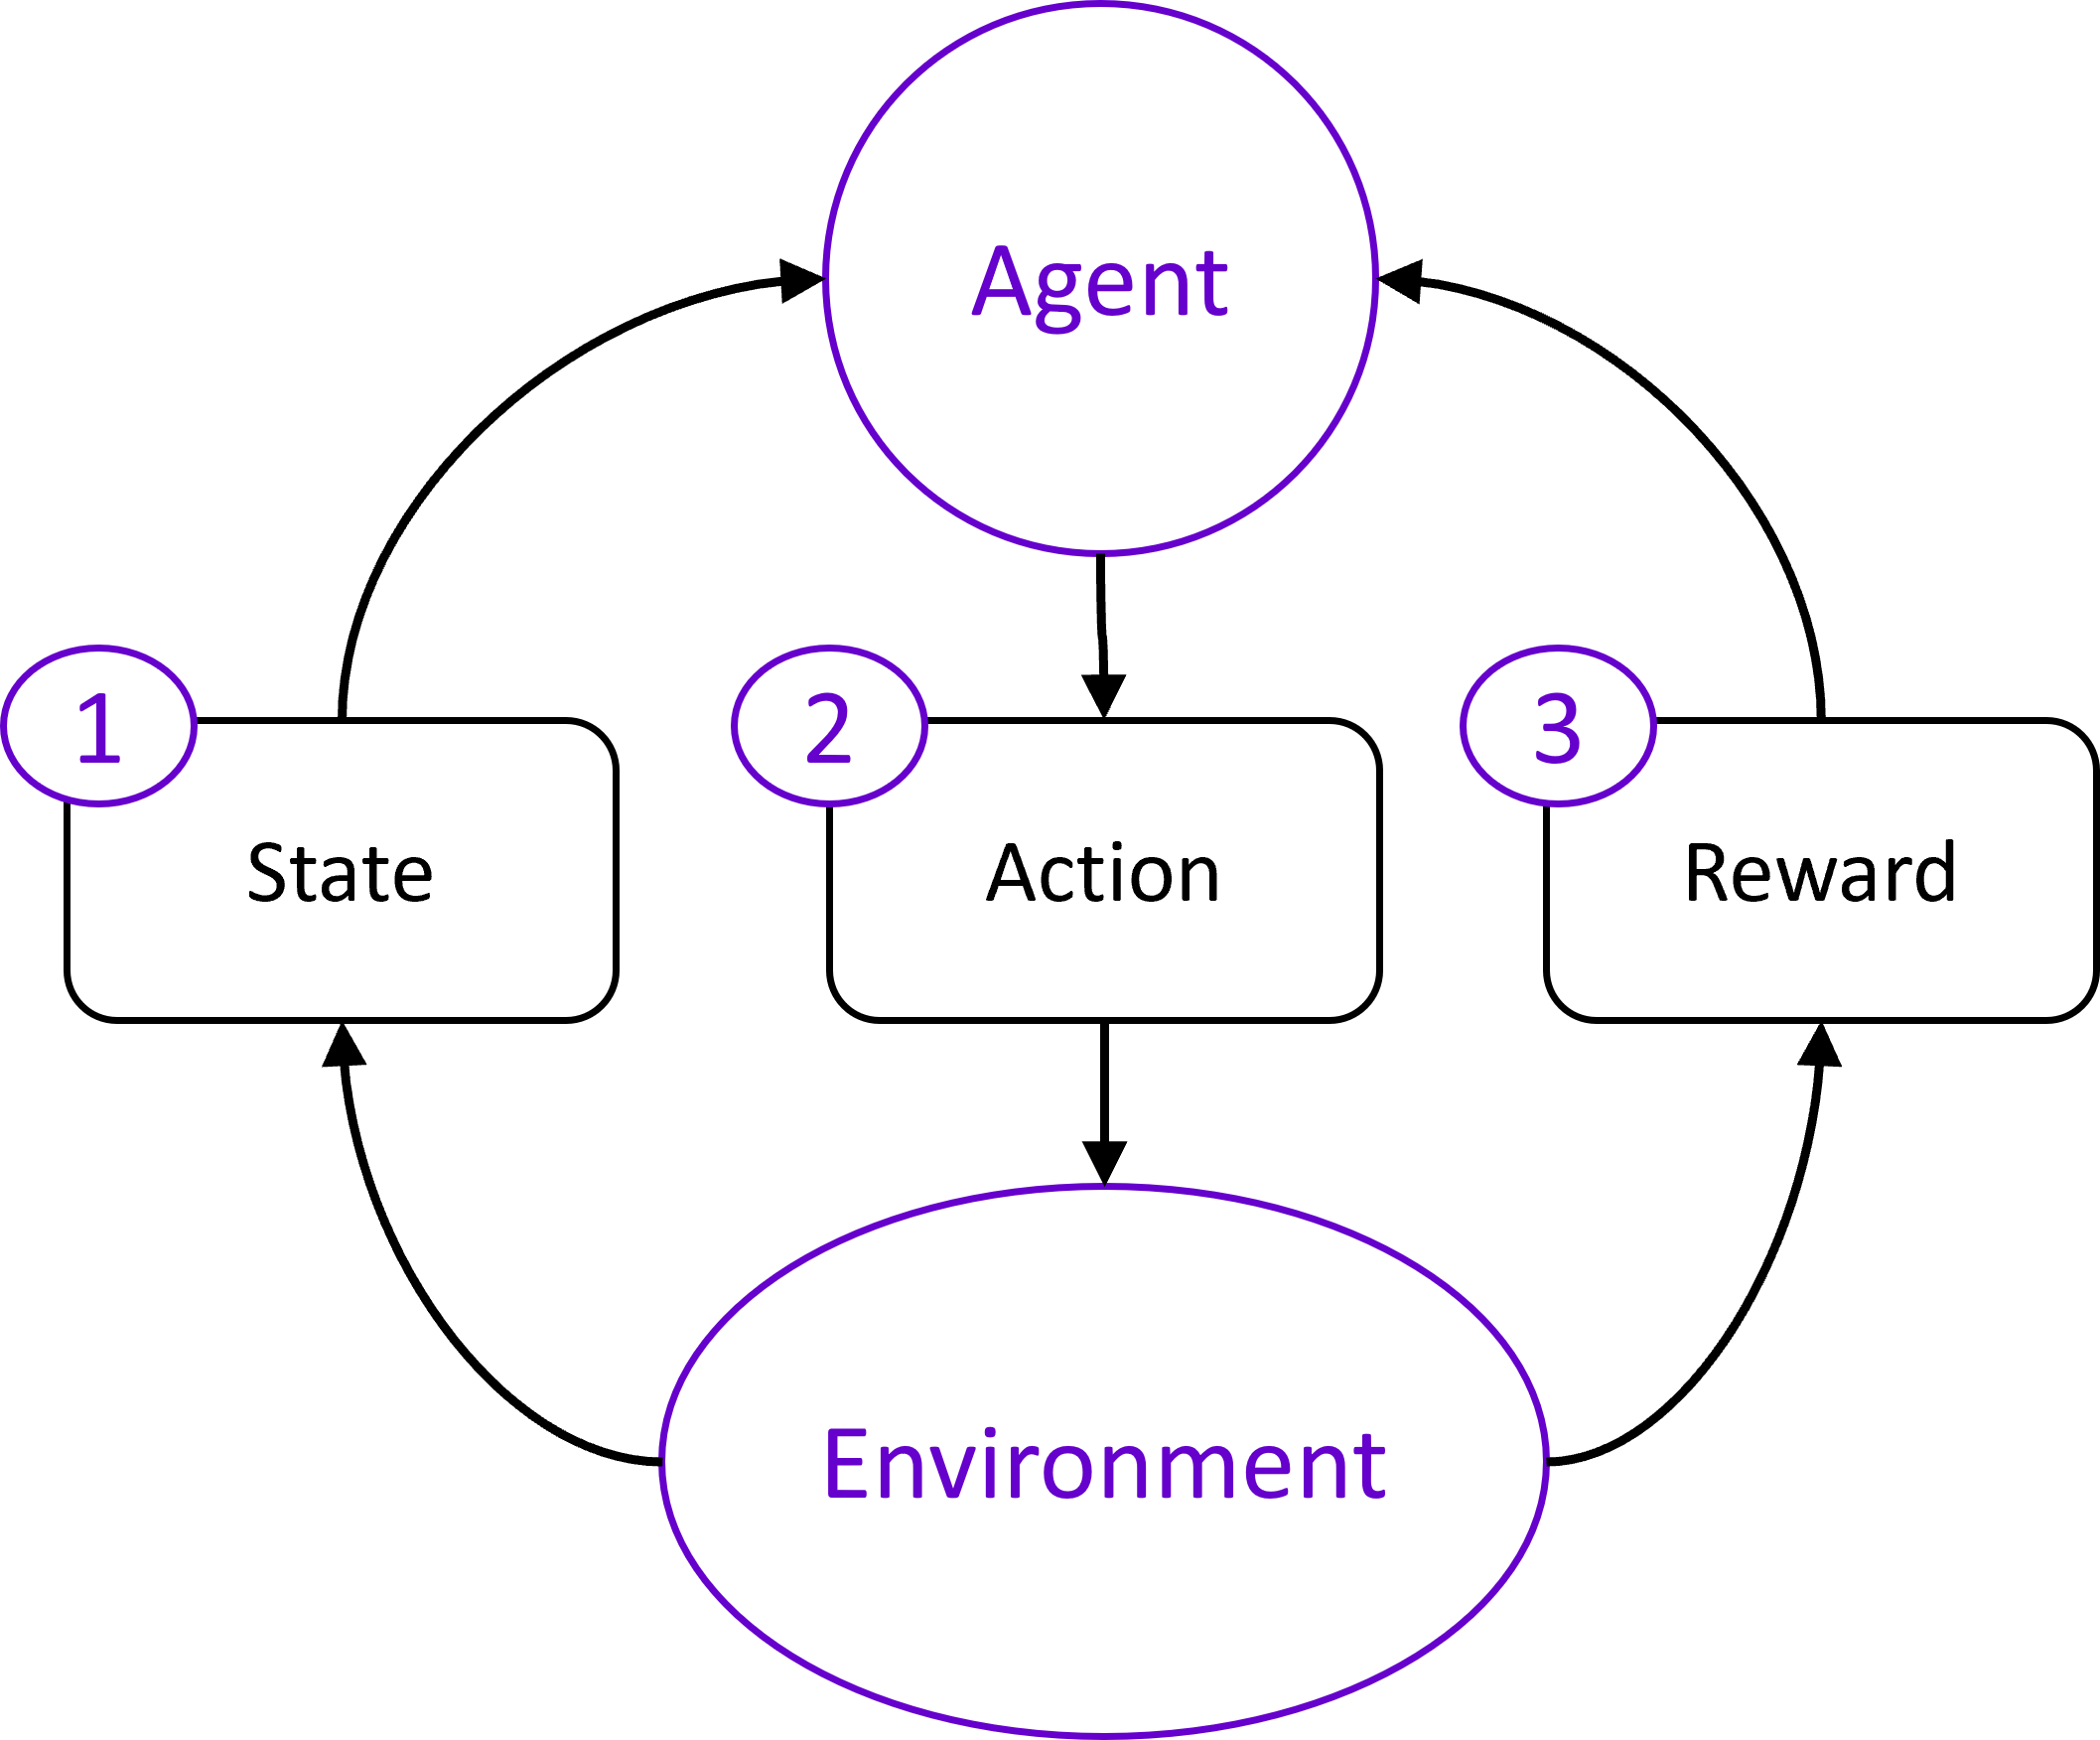
\includegraphics[width=7.5cm]{images/rl_overview.png}
  \caption [Overview of Reinforcement Learning]
  {Overview of Reinforcement Learning
  }
  \label{fig:rl_overview_diagram}
\end{figure}

\section{Value Optimization vs Policy Optimization}
Value optimization algorithms optimize the value function that predict the expected reward based on given states and actions. Value optimization algorithms face significant challenges for continuous action spaces since the output space of the value function will be enormous.
\par
Policy optimization algorithms optimize the policy, the agent's strategy to perform the action that maximizes the expected reward based on the state. Policy optimization algorithms are simpler for continuous action space as the policy can directly output continuous actions.
\section{On-policy vs Off-policy}
On-policy algorithms optimize the policy used to perform actions. But it has low sample efficiency as it requires a full episode before optimizing the parameters. 
\par
Off-policy algorithms can optimize the parameters after each step, as the optimized policy is not used to perform actions.
With the use of experience replay, Off-policy algorithms have a high sample efficiency.
\section{Deterministic Policy vs Stochastic Policy}
Deterministic policies do not explore with random actions and could trap local optima. This result could be unstable as the optimization is sensitive to the initial state.
\par
Compare to deterministic policies; stochastic policies perform random actions and favor exploration. The result is stabler as exploration will compensate for the difference of the initial state.

\section{Comparison}
After comparing the characteristics of each DRL algorithm, we choose SAC for our DRL model as it meets all of our expectations.
\begin{table}[htb]
    \centering
    \begin{tabular}{||c||c|c|c||}
    \hline\hline
        Algorithm & Value/Policy Optimization & On/Off-Policy & Determinisitc/Stochastic Policy  \\ \hline
        DQN	& Value Optimization   & \color{blue} {Off-Policy} & NA \\ \hline
        TRPO/PPO &	\color{blue} {Policy Optimization} &	On-Policy &	\color{blue} {Stochastic} \\ \hline
        DDPG/TD3 &	\color{blue} {Policy Optimization} &	\color{blue} {Off-Policy}  &	Determinisitc \\ \hline
        SAC	& \color{blue} {Policy Optimization} &	\color{blue} {Off-Policy} & \color{blue} {Stochastic} \\ \hline
    \hline\hline
    \end{tabular}
    \caption{Comparison or DRL algorithm}
    \label{tab:my_label}
\end{table}

\section{Soft Actor-Critic}
Soft Actor-Critic (SAC) is an DRL algorithm that optimizes a stochastic policy in an off-policy way with entropy regularization.
\subsection{Actor-Critic}
Actor-Critic uses both the Value Function and the Policy. The actor determines the actions with the policy. The critic uses the value function to criticize the actor's action and output the Temporal-difference (TD) error. Both the value function model and the policy model will train upon the TD error.
\begin{figure}[htb]
    \centering
    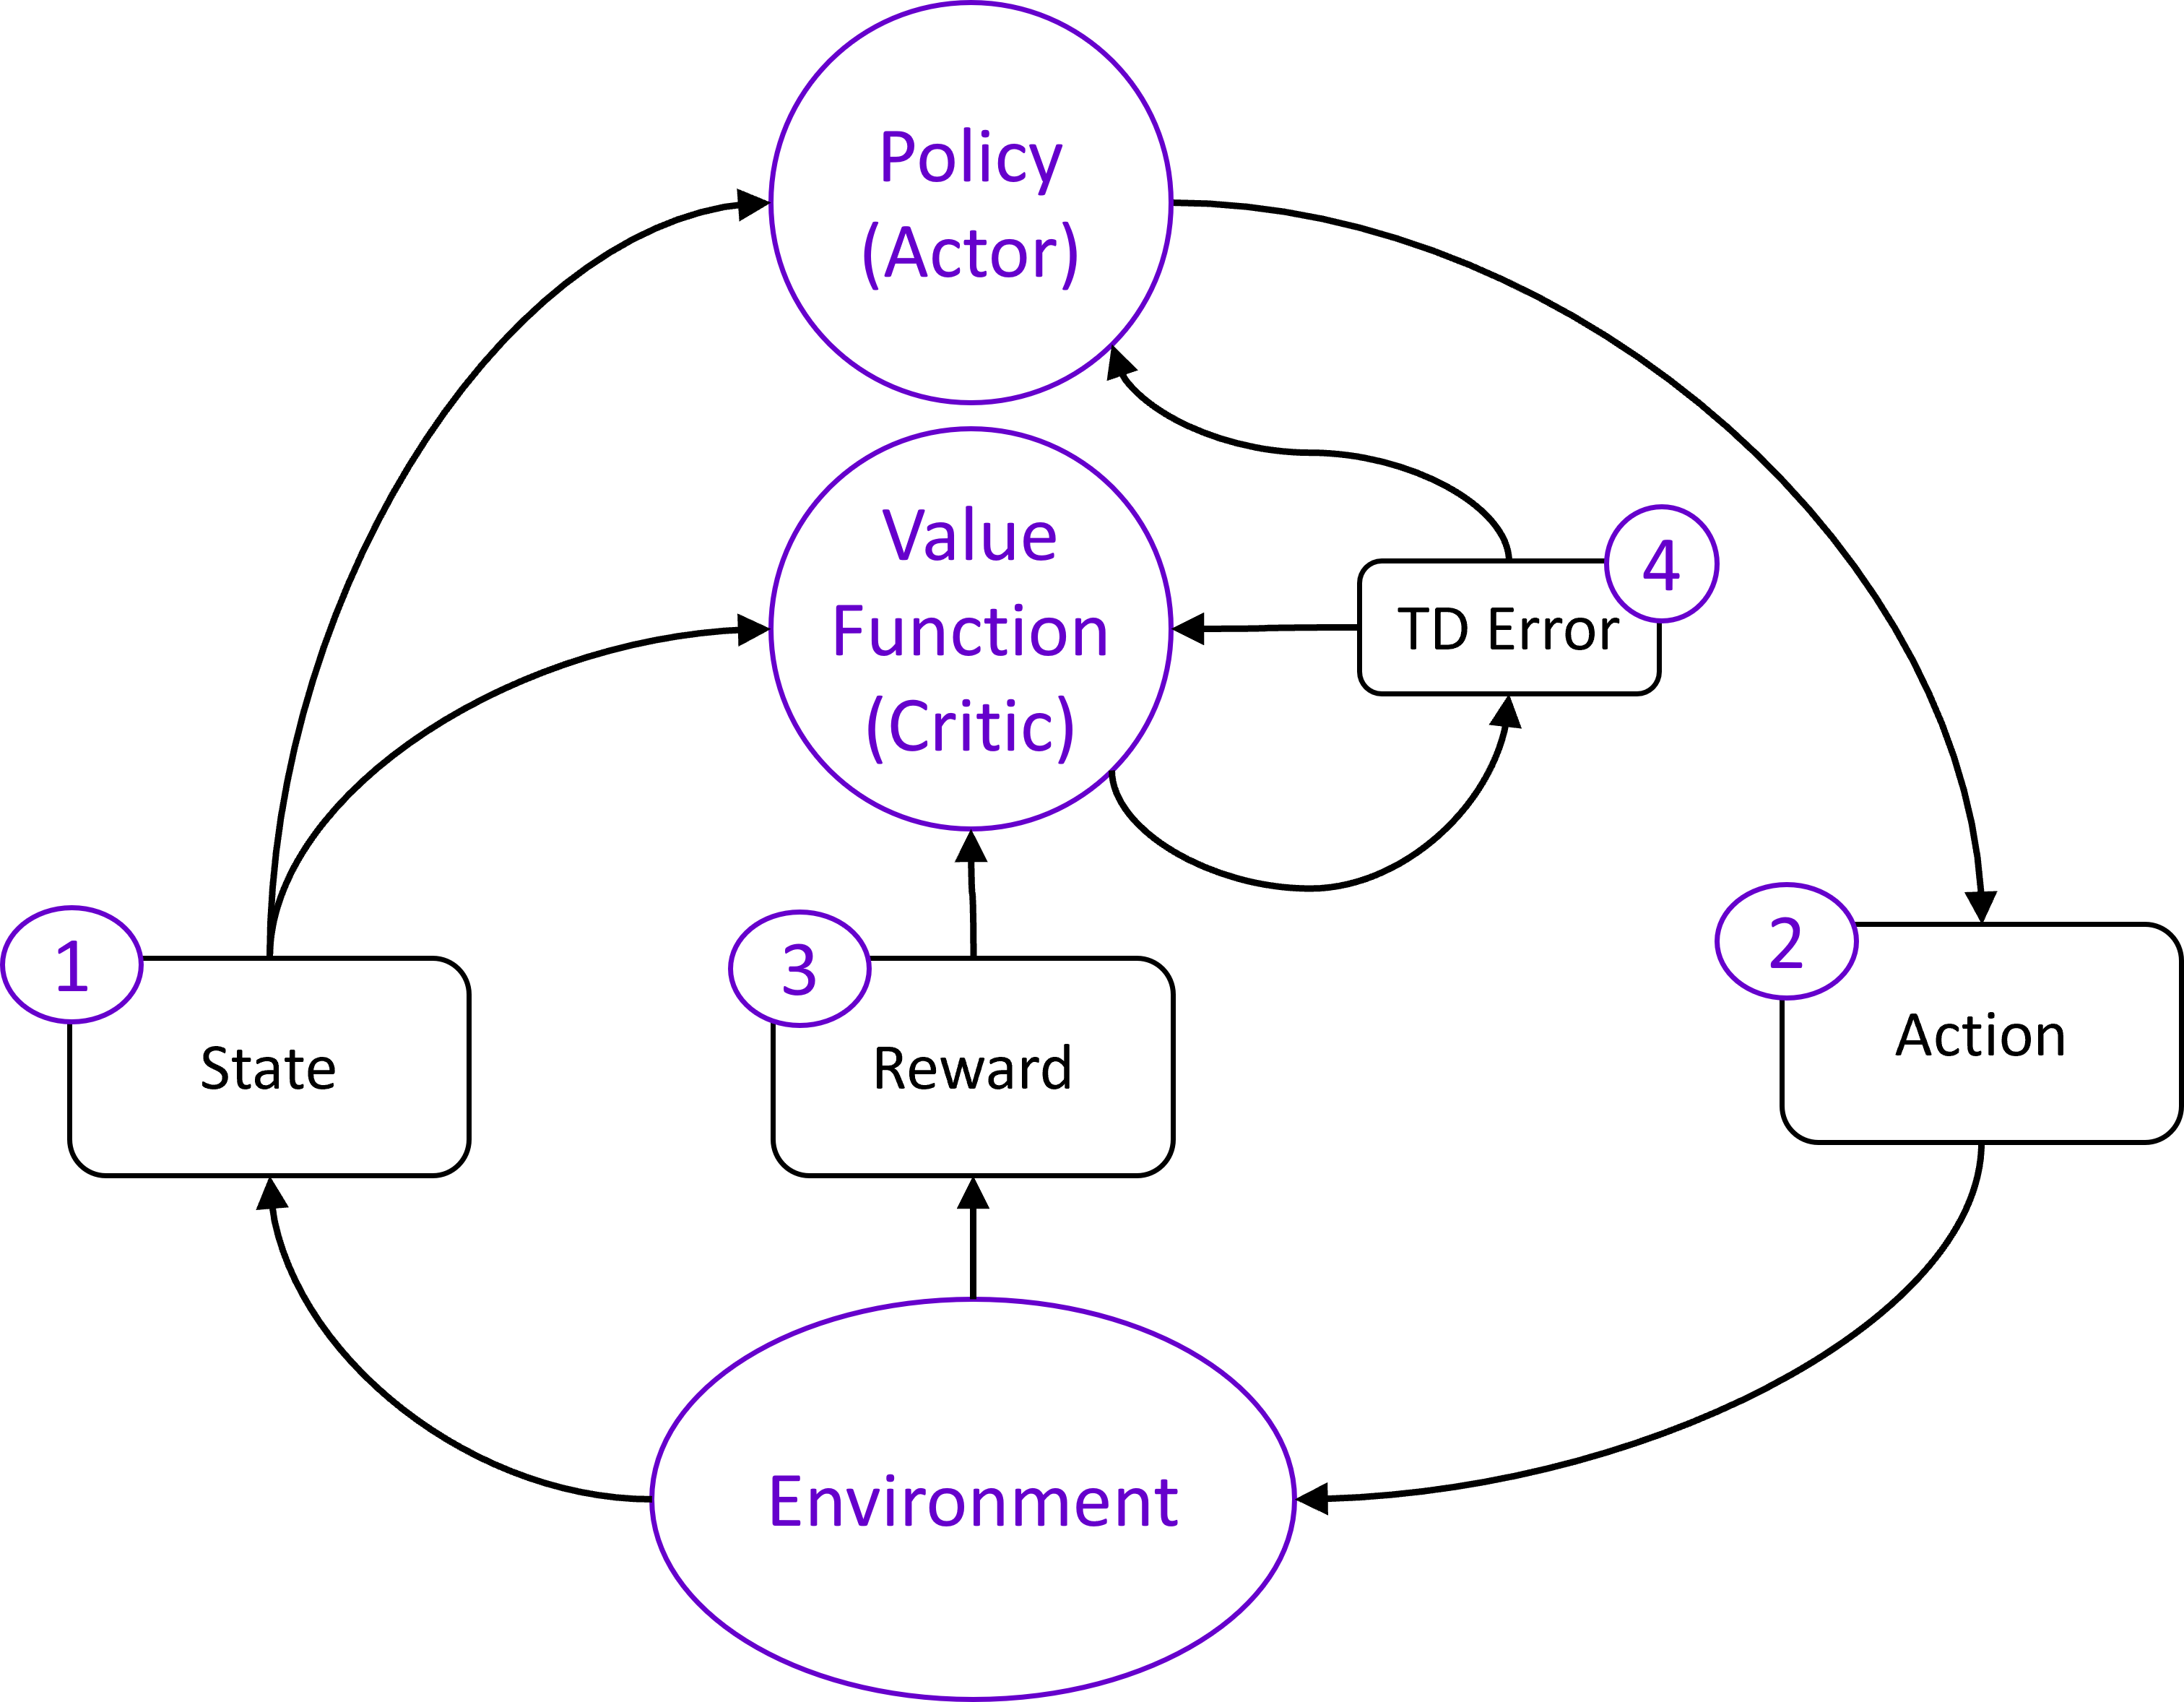
\includegraphics[width=10cm]{images/actor_critic.png}
    \caption{Actor-Critic Overview}
    \label{fig:actor-critic}
\end{figure}

\subsection{Entropy Regularization}
Entropy Regularization balances the exploration-exploitation trade-off as the algorithm favors exploration when the entropy is high initially and becomes more deterministic when entropy is low to increase exploitation.